\documentclass[a4paper]{article}

%Пакеты для математических символов:
\usepackage{amsmath} % американское математическое сообщество.
\usepackage{amssymb} % миллион разных значков и готический, ажурный шрифты.
\usepackage{amscd} % диаграммы, графики.
\usepackage{amsthm} % окружения теорем, определений и тд.
\usepackage{physics} % основные физические символы
%\usepackage{latexsym} % треугольники и пьяная стрелка.

%пакеты для шрифтов:
%\usepackage{euscript} % прописной шрифт с завитушками.
\usepackage{MnSymbol} % Значеки доказательства
\usepackage{verbatim} % улучшенный шрифт "пишущей машинки".
%\usepackage{array} % более удобные таблицы.
%\usepackage{multirow} % мультистолбцы в таблицах.
%\usepackage{longtable} % таблицы на несколько страниц.
%\usepackage{latexsym}

\usepackage{etoolbox}
\usepackage{slashbox} %Разделениени текста \backslashbox{}{}
\usepackage{collectbox} % Добавляет коробочки, можно складывать туда текст)

%Пакеты для оформления:
\RequirePackage[center, medium]{titlesec}% Стиль секций и заголовков
%\usepackage[x11names]{xcolor} % 317 новых цветов для текста.
%\usepackage{multicol} % набор текста в несколько колонн.
\usepackage{graphicx} % расширенные возможности вставки стандартных картинок.
\usepackage{subcaption} % возможность вставлять картинки в строчку
%\usepackage{caption} % возможность подавить нумерацию у caption.
\usepackage{wrapfig} % вставка картинок и таблиц, обтекаемых текстом.
\usepackage{cancel} % значки для сокращения дробей, упрощения, стремления.
\usepackage{misccorr} % в заголовках появляется точка, но при ссылке на них ее нет.
%\usepackage{indentfirst} % отступ у первой строки раздела
%\usepackage{showkeys} % показывает label формул над их номером.
%\usepackage{fancyhdr} % удобное создание верхних и нижних колонтитулов.
%\usepackage{titlesec} % еще одно создание верхних и нижних колонтитулов

\usepackage{hyperref} % Ссылки как внешние так и внутренние
\hypersetup{
    colorlinks=true,
    linkcolor=red,
    filecolor=magenta,      
    urlcolor=cyan,
    pdftitle={Overleaf Example},
    pdfpagemode=FullScreen,
    }

%Пакеты шрифтов, кодировок. НЕ МЕНЯТЬ РАСПОЛОЖЕНИЕ.
\usepackage[utf8]{inputenc} % кодировка символов.
%\usepackage{mathtext} % позволяет использовать русские буквы в формулах. НЕСОВМЕСТИМО С tempora.
\usepackage[T1, T2A]{fontenc} % кодировка шрифта.
\usepackage[english, russian]{babel} % доступные языки.


%tikz:
\usepackage{tikz} % tikz
\usetikzlibrary{decorations.text} % позволяет делать текст вдоль кривой.
\usetikzlibrary{external} % позволяет кэшировать рисунки tikz.

%Отступы и поля:
%размеры страницы А4 11.7x8.3in
\textwidth=7.3in % ширина текста
\textheight=10in % высота текста
\oddsidemargin=-0.5in % левый отступ(базовый 1дюйм + значение)
\topmargin=-0.5in % отступ сверху до колонтитула(базовый 1дюйм + значение)


%Сокращения
%Скобочки
\newcommand{\inrad}[1]{\left( #1 \right)}
\newcommand{\inner}[1]{\left( #1 \right)}
\newcommand{\infig}[1]{\left{ #1 \right}}
\newcommand{\insqr}[1]{\left[ #1 \right]}
\newcommand{\ave}[1]{\left\langle #1 \right\rangle}


%% Красивые <= и >=
\renewcommand{\geq}{\geqslant}
\renewcommand{\leq}{\leqslant}

%%Значек выполнятся
\newcommand{\per}{\hookrightarrow}


%% Более привычные греческие буквы
\renewcommand{\phi}{\varphi}
\renewcommand{\epsilon}{\varepsilon}
\newcommand{\eps}{\varepsilon}
\newcommand{\com}{\mathbb{C}}
\newcommand{\re}{\mathbb{R}}
\newcommand{\nat}{\mathbb{N}}
\newcommand{\stp}{$\filledmedtriangleleft$}
\newcommand{\enp}{$\filledmedsquare$}

\makeatletter
\newcommand{\sqbox}{%
    \collectbox{%
        \@tempdima=\dimexpr\width-\totalheight\relax
        \ifdim\@tempdima<\z@
            \fbox{\hbox{\hspace{-.5\@tempdima}\BOXCONTENT\hspace{-.5\@tempdima}}}%
        \else
            \ht\collectedbox=\dimexpr\ht\collectedbox+.5\@tempdima\relax
            \dp\collectedbox=\dimexpr\dp\collectedbox+.5\@tempdima\relax
            \fbox{\BOXCONTENT}%
        \fi
    }%
}
\makeatother
\newcommand{\mergelines}[2]{
\begin{tabular}{llp{.5\textwidth}}
#1 \\ #2
\end{tabular}
}
\newcommand\tab[1][0.51cm]{\hspace*{#1}}
\newcommand\difh[2]{\frac{\partial #1}{\partial #2}}
\newcommand{\messageforpeople}[1]{HSE Faculty of Physics \ \ HSE Faculty of Physics HSE Faculty of Physics \ \ HSE Faculty of Physics HSE Faculty of Physics \ \ HSE Faculty of Physics HSE Faculty of Physics \ \ HSE Faculty of Physics HSE Faculty of Physics \ \ HSE Faculty of Physics HSE Faculty of Physics \ \ HSE Faculty of Physics HSE Faculty of Physics \ \ HSE Faculty of Physics HSE Faculty of Physics \ \ HSE Faculty of Physics }


\numberwithin{equation}{section}

\begin{document}

\pagestyle{empty}
\oddsidemargin=-1.18in
\topmargin=-1.5in

%\begin{titlepage}
%\begin{tikzpicture}
    \draw [white] (0, 0) ellipse (4.1in and 5.7in);
    \path [postaction={
    decoration={text along path,
    text={\messageforpeople{}},
    text align=center,
    raise=0mm,
    reverse path}, decorate}]
    [postaction={
    decoration={text along path,
    text={\messageforpeople{}},
    text align=center,
    raise=3mm,
    reverse path}, decorate}]
    [postaction={
    decoration={text along path,
    text={\messageforpeople{}},
    text align=center,
    raise=6mm,
    reverse path}, decorate}]
    [postaction={
    decoration={text along path,
    text={\messageforpeople{}},
    text align=center,
    raise=9mm,
    reverse path}, decorate}]
    [postaction={
    decoration={text along path,
    text={\messageforpeople{}},
    text align=center,
    raise=12mm,
    reverse path}, decorate}] 
    [postaction={
    decoration={text along path,
    text={\messageforpeople{}},
    text align=center,
    raise=15mm,
    reverse path}, decorate}]
    [postaction={
    decoration={text along path,
    text={\messageforpeople{}},
    text align=center,
    raise=18mm,
    reverse path}, decorate}]
    [postaction={
    decoration={text along path,
    text={\messageforpeople{}},
    text align=center,
    raise=21mm,
    reverse path}, decorate}] 
    [postaction={
    decoration={text along path,
    text={\messageforpeople{}},
    text align=center,
    raise=24mm,
    reverse path}, decorate}]
    [postaction={
    decoration={text along path,
    text={\messageforpeople{}},
    text align=center,
    raise=27mm,
    reverse path}, decorate}]
    [postaction={
    decoration={text along path,
    text={\messageforpeople{}},
    text align=center,
    raise=30mm,
    reverse path}, decorate}] 
    [postaction={
    decoration={text along path,
    text={\messageforpeople{}},
    text align=center,
    raise=33mm,
    reverse path}, decorate}]
    [postaction={
    decoration={text along path,
    text={\messageforpeople{}},
    text align=center,
    raise=36mm,
    reverse path}, decorate}]
    [postaction={
    decoration={text along path,
    text={\messageforpeople{}},
    text align=center,
    raise=39mm,
    reverse path}, decorate}] 
    [postaction={
    decoration={text along path,
    text={\messageforpeople{}},
    text align=center,
    raise=42mm,
    reverse path}, decorate}]
    [postaction={
    decoration={text along path,
    text={\messageforpeople{}},
    text align=center,
    raise=45mm,
    reverse path}, decorate}]
    [postaction={
    decoration={text along path,
    text={\messageforpeople{}},
    text align=center,
    raise=48mm,
    reverse path}, decorate}] 
    [postaction={
    decoration={text along path,
    text={\messageforpeople{}},
    text align=center,
    raise=51mm,
    reverse path}, decorate}]
    [postaction={
    decoration={text along path,
    text={\messageforpeople{}},
    text align=center,
    raise=54mm,
    reverse path}, decorate}]
    [postaction={
    decoration={text along path,
    text={\messageforpeople{}},
    text align=center,
    raise=57mm,
    reverse path}, decorate}] 
    [postaction={
    decoration={text along path,
    text={\messageforpeople{}},
    text align=center,
    raise=60mm,
    reverse path}, decorate}]
    [postaction={
    decoration={text along path,
    text={\messageforpeople{}},
    text align=center,
    raise=63mm,
    reverse path}, decorate}]
    [postaction={
    decoration={text along path,
    text={\messageforpeople{}},
    text align=center,
    raise=66mm,
    reverse path}, decorate}] 
    [postaction={
    decoration={text along path,
    text={\messageforpeople{}},
    text align=center,
    raise=69mm,
    reverse path}, decorate}]
    [postaction={
    decoration={text along path,
    text={\messageforpeople{}},
    text align=center,
    raise=72mm,
    reverse path}, decorate}]
    (0, 0) ellipse (2.75in and 4.96in);
    \node at (0, 3.2in) {\Large\textbf{Лабораторная по химии номер 2}};
    \node at (0, 0in) {
\includegraphics[height=4in]{FOPF.png}};
    \node at (0, -3in) {Авторы:};
    \node at (0, -3.2in) {Карибджанов Матвей};
    \node at (0, -3.5in) {February 2023};
\end{tikzpicture}

%2.75in and 4.96in
%\end{titlepage}

\oddsidemargin=-0.5in
\topmargin=-0.5in
\pagestyle{plain}

\newpage
\tikzexternalize
\tableofcontents
\newpagestyle{main}{
\setfootrule{0.4pt}
\setfoot{}{\thepage}{\sectiontitle}}
\pagestyle{main}

\section{Эксперемент}

\subsection{Часть}

Используя формулу Нерста: 

\begin{equation}
  E = E_0 - \cfrac{RT}{Fz}\ln\inner{\cfrac{a_{r}}{a_o}}  
\end{equation}

Примем $R = 8.81, \ F = 9.64\cdot10^4, T = 300^{\circ}F$

\begin{eqnarray}
  ZnSO_4 &\to& Zn^{2+} + SO_4^{2-} \\
  CuSO_4 &\to& Cu^{2+} + SO_4^{2-}
\end{eqnarray}

Пот таблице стандартный эл. потенциалов
 $E_{0Zn} = -0.763, \ E_{0Cu} = 0.337 $











\section{Пропускающая решетка}
Рассмотрим:
\begin{equation}
    \insqr{\cfrac{\sin\inner{\cfrac{kb}{2}\sin{x}}}{\cfrac{kb}{2}\sin{x}}
    \cfrac{\sin\inner{N\cfrac{kd}{2}\sin{x}}}{\sin\inner{\cfrac{kd}{2}\sin{x}}}}^2
\end{equation}

Из определения $d, b$ заметим что $d \geq b$ откуда следует, что
\begin{equation}
    \insqr{\cfrac{\sin\inner{N\cfrac{kd}{2}\sin{x}}}{\sin\inner{\cfrac{kd}{2}\sin{x}}}}^2
\end{equation}

будет огибающей. Следовательно максимумы будут задаваться 

\begin{equation}
    \insqr{\cfrac{\sin\inner{\cfrac{kb}{2}\sin{x}}}{\cfrac{kb}{2}\sin{x}}}^2
\end{equation}

\begin{figure}[h]
    \centering
    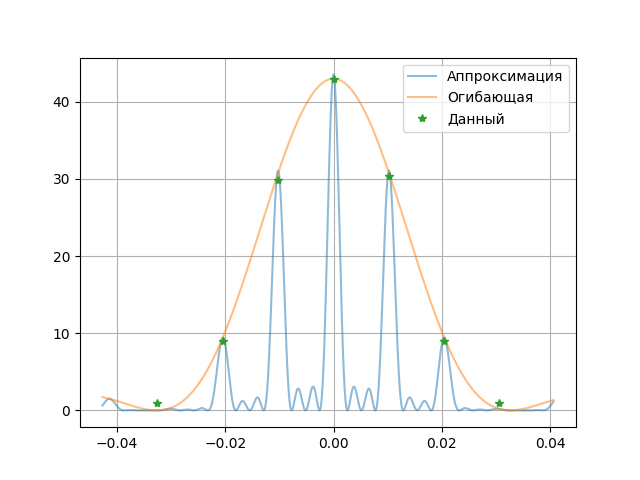
\includegraphics[trim={0 0 0 0},clip,width=\textwidth]{Ex_2/ex_2_1.png}
    \caption{}
    \label{Ex_2_1}
\end{figure}

$d$ нахожу как среднее по формуле:
\begin{equation}
    d\sin{x} = n\lambda
\end{equation}
где $x$ это расположения максимумов, а $n$ номер соответствующего максимума.

$b$ это будет 
\begin{equation}
    b\sin{x} = \lambda,
\end{equation}
так как 
\begin{equation}
    \sin\inner{\cfrac{kb}{2}\sin{x}} = 0
\end{equation}

В итоге я получил $d = 5.16 nm, b = 1.63 nm$





\end{document}